\documentclass[border=5pt]{standalone}
\usepackage[T1]{fontenc}
\usepackage{lmodern}
\usepackage{pgfplots}
\usepgfplotslibrary{groupplots}
\pgfplotsset{compat=1.18}
\begin{document}
\sffamily
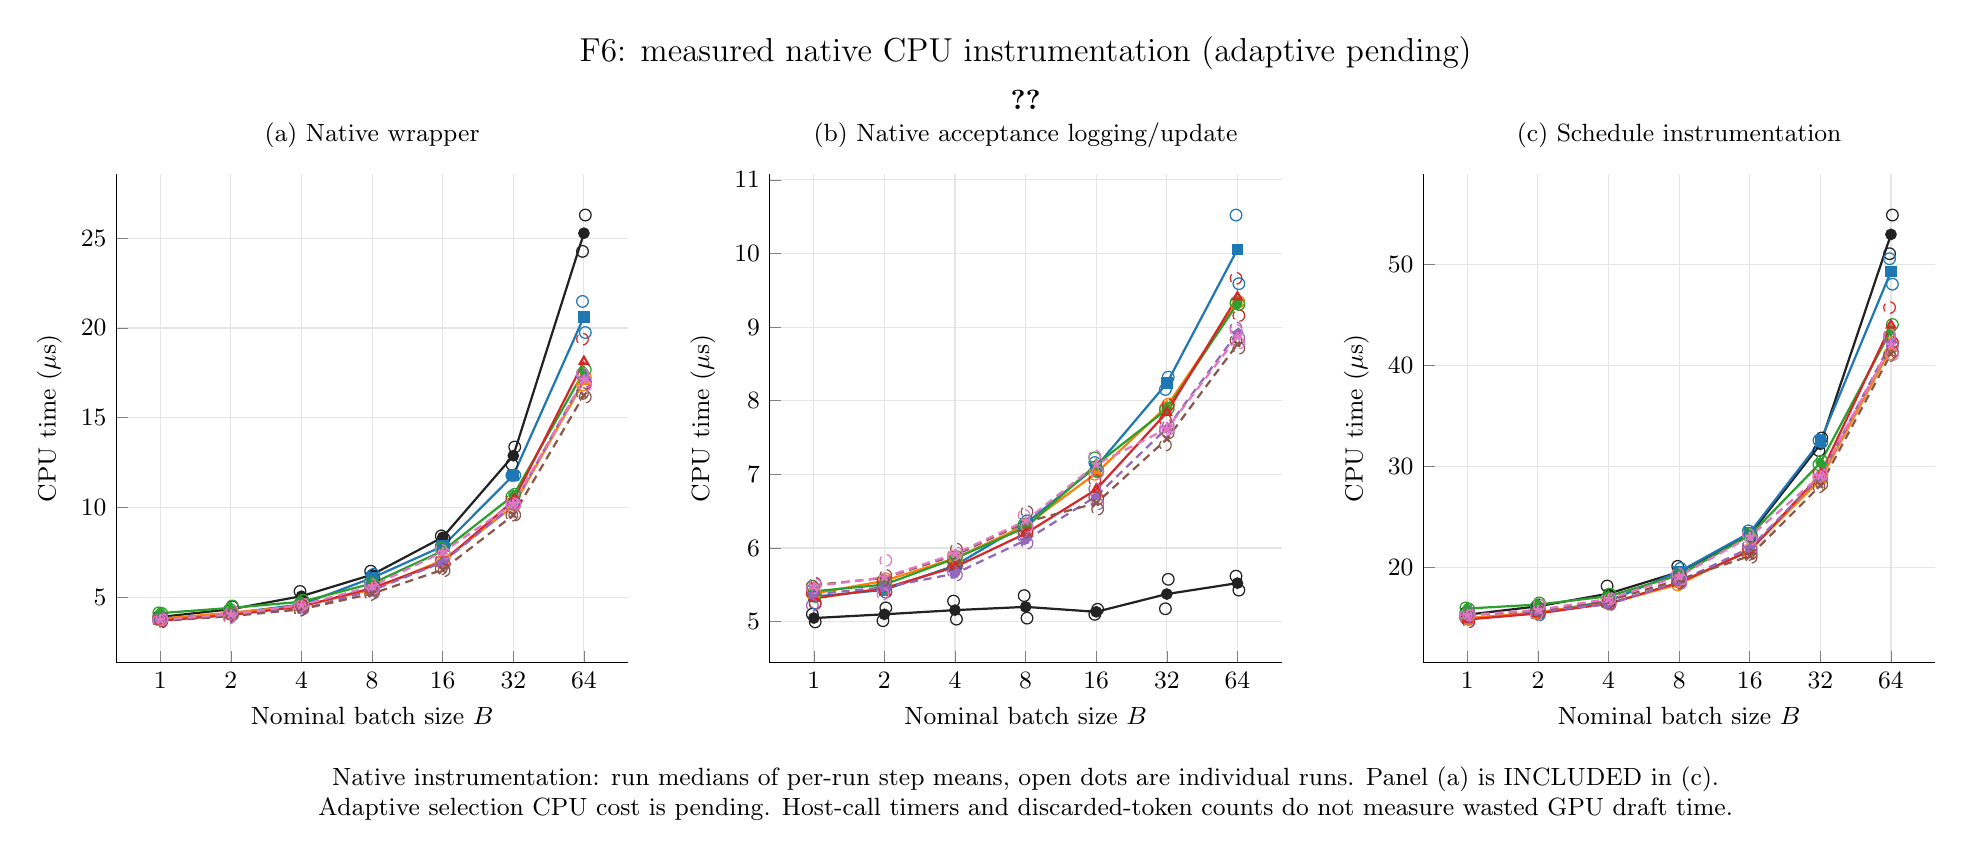
\begin{tikzpicture}
\definecolor{series0}{HTML}{222222}
\definecolor{series1}{HTML}{1f77b4}
\definecolor{series2}{HTML}{ff7f0e}
\definecolor{series3}{HTML}{2ca02c}
\definecolor{series4}{HTML}{d62728}
\definecolor{series5}{HTML}{9467bd}
\definecolor{series6}{HTML}{8c564b}
\definecolor{series7}{HTML}{e377c2}
\begin{groupplot}[group style={group size=3 by 1,horizontal sep=1.8cm},width=6.5cm,height=6.2cm,scale only axis,grid=major,grid style={gray!20},axis lines*=left,tick label style={font=\small},label style={font=\small},title style={font=\small},unbounded coords=jump]
\nextgroupplot[title={(a) Native wrapper},xlabel={Nominal batch size $B$},ylabel={CPU time ($\mu$s)},xtick={1,2,4,8,16,32,64},xticklabels={1,2,4,8,16,32,64},xmode=log,log basis x=2,minor x tick num=0,scaled y ticks=false,yticklabel style={/pgf/number format/fixed,/pgf/number format/precision=2},legend columns=8,legend to name=sharedlegend,legend style={draw=none,font=\small,/tikz/every even column/.append style={column sep=8pt}}]
\addplot+[color=series0,mark=*,mark size=1.7pt,mark options={fill=series0,draw=series0},line width=0.8pt] coordinates {(1,3.91078094242) (2,4.34066560039) (4,5.06836515748) (8,6.26557431102) (16,8.34681692913) (32,12.888738189) (64,25.2749094488)};
\addlegendentry{$\gamma=0$}
\addplot+[only marks,forget plot,color=series0,mark=o,mark size=2.1pt,mark options={fill=white,line width=0.45pt}] coordinates {(0.986097544263,3.91672588583) (1.01409845894,3.90483599902) (1.97219508853,4.19913139764) (2.02819691788,4.48219980315) (3.94439017705,5.33051230315) (4.05639383575,4.80621801181) (7.8887803541,6.45887795276) (8.11278767151,6.07227066929) (15.7775607082,8.42468700787) (16.225575343,8.26894685039) (31.5551214164,12.4057677165) (32.451150686,13.3717086614) (63.1102428328,24.2640708661) (64.9023013721,26.2857480315)};
\addplot+[color=series1,mark=square*,mark size=1.7pt,mark options={fill=series1,draw=series1},line width=0.8pt] coordinates {(1,3.78735175202) (2,4.11533424479) (4,4.60620967742) (8,6.08409031282) (16,7.84724251497) (32,11.7955657371) (64,20.6119722222)};
\addlegendentry{$\gamma=1$}
\addplot+[only marks,forget plot,color=series1,mark=o,mark size=2.1pt,mark options={fill=white,line width=0.45pt}] coordinates {(0.986097544263,3.8486319407) (1.01409845894,3.72607156334) (1.97219508853,4.16790390625) (2.02819691788,4.06276458333) (3.94439017705,4.60726932924) (4.05639383575,4.6051500256) (7.8887803541,5.8884974773) (8.11278767151,6.27968314834) (15.7775607082,7.84388622754) (16.225575343,7.8505988024) (31.5551214164,11.7916772908) (32.451150686,11.7994541833) (63.1102428328,21.477) (64.9023013721,19.7469444444)};
\addplot+[color=series2,mark=triangle*,mark size=1.7pt,mark options={fill=series2,draw=series2},line width=0.8pt] coordinates {(1,3.81604490644) (2,4.14372513228) (4,4.51809751681) (8,5.43943813387) (16,7.06972389558) (32,10.07415) (64,17.0273849206)};
\addlegendentry{$\gamma=2$}
\addplot+[only marks,forget plot,color=series2,mark=o,mark size=2.1pt,mark options={fill=white,line width=0.45pt}] coordinates {(0.986097544263,3.78924823285) (1.01409845894,3.84284158004) (1.97219508853,4.07854285714) (2.02819691788,4.20890740741) (3.94439017705,4.53279772375) (4.05639383575,4.50339730988) (7.8887803541,5.42797768763) (8.11278767151,5.45089858012) (15.7775607082,6.97313855422) (16.225575343,7.16630923695) (31.5551214164,10.02182) (32.451150686,10.12648) (63.1102428328,16.8189603175) (64.9023013721,17.2358095238)};
\addplot+[color=series3,mark=diamond*,mark size=1.7pt,mark options={fill=series3,draw=series3},line width=0.8pt] coordinates {(1,4.12370256806) (2,4.41439978706) (4,4.75695246753) (8,5.77452446483) (16,7.59169919517) (32,10.672248) (64,17.5698452381)};
\addlegendentry{$\gamma=3$}
\addplot+[only marks,forget plot,color=series3,mark=o,mark size=2.1pt,mark options={fill=white,line width=0.45pt}] coordinates {(0.986097544263,4.1385931799) (1.01409845894,4.10881195622) (1.97219508853,4.30560340697) (2.02819691788,4.52319616715) (3.94439017705,4.67136363636) (4.05639383575,4.8425412987) (7.8887803541,5.81967482161) (8.11278767151,5.72937410805) (15.7775607082,7.73544668008) (16.225575343,7.44795171026) (31.5551214164,10.605232) (32.451150686,10.739264) (63.1102428328,17.4699444444) (64.9023013721,17.6697460317)};
\addplot+[color=series4,mark=triangle,mark size=1.7pt,mark options={fill=series4,draw=series4},line width=0.8pt] coordinates {(1,3.70728229226) (2,4.01801390003) (4,4.497509375) (8,5.51895714286) (16,6.97703846154) (32,10.3707791165) (64,18.1360039683)};
\addlegendentry{$\gamma=4$}
\addplot+[only marks,forget plot,color=series4,mark=o,mark size=2.1pt,mark options={fill=white,line width=0.45pt}] coordinates {(0.986097544263,3.77706670435) (1.01409845894,3.63749788016) (1.97219508853,3.9738698209) (2.02819691788,4.06215797915) (3.94439017705,4.47870989583) (4.05639383575,4.51630885417) (7.8887803541,5.45211326531) (8.11278767151,5.58580102041) (15.7775607082,7.08655668016) (16.225575343,6.86752024291) (31.5551214164,10.4302931727) (32.451150686,10.3112650602) (63.1102428328,19.3762301587) (64.9023013721,16.8957777778)};
\addplot+[color=series5,mark=pentagon*,mark size=1.7pt,mark options={fill=series5,draw=series5},line width=0.8pt] coordinates {(1,3.78319269504) (2,4.04839557641) (4,4.33753675704) (8,5.38257985758) (16,6.96113636364) (32,10.1325562249) (64,17.1819087302)};
\addlegendentry{$\gamma=5$}
\addplot+[only marks,forget plot,color=series5,mark=o,mark size=2.1pt,mark options={fill=white,line width=0.45pt}] coordinates {(0.986097544263,3.69511404255) (1.01409845894,3.87127134752) (1.97219508853,4.02543029491) (2.02819691788,4.07136085791) (3.94439017705,4.31486704901) (4.05639383575,4.36020646507) (7.8887803541,5.39716480163) (8.11278767151,5.36799491353) (15.7775607082,7.04893333333) (16.225575343,6.87333939394) (31.5551214164,10.0388393574) (32.451150686,10.2262730924) (63.1102428328,17.3361111111) (64.9023013721,17.0277063492)};
\addplot+[color=series6,mark=x,mark size=1.7pt,mark options={fill=series6,draw=series6},line width=0.8pt] coordinates {(1,3.69247872492) (2,3.95357593239) (4,4.3400843342) (8,5.20744177732) (16,6.53944366197) (32,9.58075697211) (64,16.2545753968)};
\addlegendentry{$\gamma=6$}
\addplot+[only marks,forget plot,color=series6,mark=o,mark size=2.1pt,mark options={fill=white,line width=0.45pt}] coordinates {(0.986097544263,3.66961092927) (1.01409845894,3.71534652056) (1.97219508853,3.89032170647) (2.02819691788,4.0168301583) (3.94439017705,4.27622506527) (4.05639383575,4.40394360313) (7.8887803541,5.15968539326) (8.11278767151,5.25519816139) (15.7775607082,6.59378470825) (16.225575343,6.48510261569) (31.5551214164,9.57719521912) (32.451150686,9.5843187251) (63.1102428328,16.3533730159) (64.9023013721,16.1557777778)};
\addplot+[color=series7,mark=star,mark size=1.7pt,mark options={fill=series7,draw=series7},line width=0.8pt] coordinates {(1,3.75358094627) (2,4.05285978552) (4,4.57040224778) (8,5.61995112016) (16,7.52880661323) (32,10.204004) (64,17.1244563492)};
\addlegendentry{$\gamma=7$}
\addplot+[only marks,forget plot,color=series7,mark=o,mark size=2.1pt,mark options={fill=white,line width=0.45pt}] coordinates {(0.986097544263,3.74376542682) (1.01409845894,3.76339646573) (1.97219508853,3.84812788204) (2.02819691788,4.25759168901) (3.94439017705,4.51702613696) (4.05639383575,4.6237783586) (7.8887803541,5.72341649695) (8.11278767151,5.51648574338) (15.7775607082,7.62113026052) (16.225575343,7.43648296593) (31.5551214164,10.236824) (32.451150686,10.171184) (63.1102428328,17.4648095238) (64.9023013721,16.7841031746)};
\nextgroupplot[title={(b) Native acceptance logging/update},xlabel={Nominal batch size $B$},ylabel={CPU time ($\mu$s)},xtick={1,2,4,8,16,32,64},xticklabels={1,2,4,8,16,32,64},xmode=log,log basis x=2,minor x tick num=0,scaled y ticks=false,yticklabel style={/pgf/number format/fixed,/pgf/number format/precision=2}]
\addplot+[color=series0,mark=*,mark size=1.7pt,mark options={fill=series0,draw=series0},line width=0.8pt] coordinates {(1,5.04824753937) (2,5.09924003445) (4,5.15596776575) (8,5.2000492126) (16,5.13282874016) (32,5.37452755906) (64,5.52272440945)};
\addplot+[only marks,forget plot,color=series0,mark=o,mark size=2.1pt,mark options={fill=white,line width=0.45pt}] coordinates {(0.986097544263,5.10016978346) (1.01409845894,4.99632529528) (1.97219508853,5.01240280512) (2.02819691788,5.18607726378) (3.94439017705,5.27866781496) (4.05639383575,5.03326771654) (7.8887803541,5.35284645669) (8.11278767151,5.0472519685) (15.7775607082,5.09850787402) (16.225575343,5.1671496063) (31.5551214164,5.17442913386) (32.451150686,5.57462598425) (63.1102428328,5.61748818898) (64.9023013721,5.42796062992)};
\addplot+[color=series1,mark=square*,mark size=1.7pt,mark options={fill=series1,draw=series1},line width=0.8pt] coordinates {(1,5.33889514825) (2,5.43082096354) (4,5.76193369176) (8,6.33211150353) (16,7.10529540918) (32,8.23747011952) (64,10.0569047619)};
\addplot+[only marks,forget plot,color=series1,mark=o,mark size=2.1pt,mark options={fill=white,line width=0.45pt}] coordinates {(0.986097544263,5.42551927224) (1.01409845894,5.25227102426) (1.97219508853,5.46223776042) (2.02819691788,5.39940416667) (3.94439017705,5.73586175115) (4.05639383575,5.78800563236) (7.8887803541,6.29434409687) (8.11278767151,6.36987891019) (15.7775607082,7.16034331337) (16.225575343,7.05024750499) (31.5551214164,8.15375697211) (32.451150686,8.32118326693) (63.1102428328,10.523) (64.9023013721,9.59080952381)};
\addplot+[color=series2,mark=triangle*,mark size=1.7pt,mark options={fill=series2,draw=series2},line width=0.8pt] coordinates {(1,5.38042044352) (2,5.55448664021) (4,5.86005276772) (8,6.30730476673) (16,7.01777108434) (32,7.925626) (64,9.33263095238)};
\addplot+[only marks,forget plot,color=series2,mark=o,mark size=2.1pt,mark options={fill=white,line width=0.45pt}] coordinates {(0.986097544263,5.37951074151) (1.01409845894,5.38133014553) (1.97219508853,5.52702619048) (2.02819691788,5.58194708995) (3.94439017705,5.88025763063) (4.05639383575,5.83984790481) (7.8887803541,6.32112576065) (8.11278767151,6.29348377282) (15.7775607082,7.0022248996) (16.225575343,7.03331726908) (31.5551214164,7.898216) (32.451150686,7.953036) (63.1102428328,9.32053968254) (64.9023013721,9.34472222222)};
\addplot+[color=series3,mark=diamond*,mark size=1.7pt,mark options={fill=series3,draw=series3},line width=0.8pt] coordinates {(1,5.41140920573) (2,5.50297950492) (4,5.85779038961) (8,6.27856880734) (16,7.13313682093) (32,7.884262) (64,9.32153571429)};
\addplot+[only marks,forget plot,color=series3,mark=o,mark size=2.1pt,mark options={fill=white,line width=0.45pt}] coordinates {(0.986097544263,5.48013934886) (1.01409845894,5.34267906259) (1.97219508853,5.45932233165) (2.02819691788,5.5466366782) (3.94439017705,5.83024467532) (4.05639383575,5.8853361039) (7.8887803541,6.31778389399) (8.11278767151,6.23935372069) (15.7775607082,7.22447686117) (16.225575343,7.04179678068) (31.5551214164,7.874244) (32.451150686,7.89428) (63.1102428328,9.33384126984) (64.9023013721,9.30923015873)};
\addplot+[color=series4,mark=triangle,mark size=1.7pt,mark options={fill=series4,draw=series4},line width=0.8pt] coordinates {(1,5.31417453363) (2,5.45446057204) (4,5.74165885417) (8,6.19723826531) (16,6.79539676113) (32,7.84137951807) (64,9.41037301587)};
\addplot+[only marks,forget plot,color=series4,mark=o,mark size=2.1pt,mark options={fill=white,line width=0.45pt}] coordinates {(0.986097544263,5.38553094969) (1.01409845894,5.24281811758) (1.97219508853,5.50177118418) (2.02819691788,5.4071499599) (3.94439017705,5.731715625) (4.05639383575,5.75160208333) (7.8887803541,6.18896326531) (8.11278767151,6.20551326531) (15.7775607082,6.91950404858) (16.225575343,6.67128947368) (31.5551214164,7.73924497992) (32.451150686,7.94351405622) (63.1102428328,9.66341269841) (64.9023013721,9.15733333333)};
\addplot+[color=series5,mark=pentagon*,mark size=1.7pt,mark options={fill=series5,draw=series5},line width=0.8pt] coordinates {(1,5.37166978723) (2,5.4661613941) (4,5.65212278415) (8,6.10552797558) (16,6.7017959596) (32,7.62811445783) (64,8.92103968254)};
\addplot+[only marks,forget plot,color=series5,mark=o,mark size=2.1pt,mark options={fill=white,line width=0.45pt}] coordinates {(0.986097544263,5.22029134752) (1.01409845894,5.52304822695) (1.97219508853,5.43093887399) (2.02819691788,5.50138391421) (3.94439017705,5.67062200209) (4.05639383575,5.63362356621) (7.8887803541,6.14547609359) (8.11278767151,6.06557985758) (15.7775607082,6.80463636364) (16.225575343,6.59895555556) (31.5551214164,7.59500803213) (32.451150686,7.66122088353) (63.1102428328,8.9896984127) (64.9023013721,8.85238095238)};
\addplot+[color=series6,mark=x,mark size=1.7pt,mark options={fill=series6,draw=series6},line width=0.8pt] coordinates {(1,5.49510694464) (2,5.59363858331) (4,5.90069765013) (8,6.35137027579) (16,6.6089527163) (32,7.48042031873) (64,8.76792460317)};
\addplot+[only marks,forget plot,color=series6,mark=o,mark size=2.1pt,mark options={fill=white,line width=0.45pt}] coordinates {(0.986097544263,5.4801122812) (1.01409845894,5.51010160808) (1.97219508853,5.5600110008) (2.02819691788,5.62726616582) (3.94439017705,5.81705848564) (4.05639383575,5.98433681462) (7.8887803541,6.20949131767) (8.11278767151,6.49324923391) (15.7775607082,6.6894889336) (16.225575343,6.52841649899) (31.5551214164,7.39803585657) (32.451150686,7.56280478088) (63.1102428328,8.82118253968) (64.9023013721,8.71466666667)};
\addplot+[color=series7,mark=star,mark size=1.7pt,mark options={fill=series7,draw=series7},line width=0.8pt] coordinates {(1,5.4797244549) (2,5.60321032172) (4,5.92004521694) (8,6.36892617108) (16,7.13540781563) (32,7.619422) (64,8.8706468254)};
\addplot+[only marks,forget plot,color=series7,mark=o,mark size=2.1pt,mark options={fill=white,line width=0.45pt}] coordinates {(0.986097544263,5.45667493231) (1.01409845894,5.50277397748) (1.97219508853,5.37404343164) (2.02819691788,5.8323772118) (3.94439017705,5.90613329848) (4.05639383575,5.93395713539) (7.8887803541,6.4442311609) (8.11278767151,6.29362118126) (15.7775607082,7.24798797595) (16.225575343,7.02282765531) (31.5551214164,7.626596) (32.451150686,7.612248) (63.1102428328,8.95788888889) (64.9023013721,8.7834047619)};
\nextgroupplot[title={(c) Schedule instrumentation},xlabel={Nominal batch size $B$},ylabel={CPU time ($\mu$s)},xtick={1,2,4,8,16,32,64},xticklabels={1,2,4,8,16,32,64},xmode=log,log basis x=2,minor x tick num=0,scaled y ticks=false,yticklabel style={/pgf/number format/fixed,/pgf/number format/precision=2}]
\addplot+[color=series0,mark=*,mark size=1.7pt,mark options={fill=series0,draw=series0},line width=0.8pt] coordinates {(1,15.3182085384) (2,16.1489980315) (4,17.4003624508) (8,19.5416373031) (16,23.2043572835) (32,32.173246063) (64,52.9353307087)};
\addplot+[only marks,forget plot,color=series0,mark=o,mark size=2.1pt,mark options={fill=white,line width=0.45pt}] coordinates {(0.986097544263,15.5025520423) (1.01409845894,15.1338650344) (1.97219508853,16.0313937008) (2.02819691788,16.2666023622) (3.94439017705,18.1548380906) (4.05639383575,16.645886811) (7.8887803541,20.1011240157) (8.11278767151,18.9821505906) (15.7775607082,23.3186811024) (16.225575343,23.0900334646) (31.5551214164,31.5500393701) (32.451150686,32.7964527559) (63.1102428328,51.0235275591) (64.9023013721,54.8471338583)};
\addplot+[color=series1,mark=square*,mark size=1.7pt,mark options={fill=series1,draw=series1},line width=0.8pt] coordinates {(1,14.9582131402) (2,15.4667183594) (4,16.6771157194) (8,19.5719707366) (16,23.4271836327) (32,32.4778824701) (64,49.2683134921)};
\addplot+[only marks,forget plot,color=series1,mark=o,mark size=2.1pt,mark options={fill=white,line width=0.45pt}] coordinates {(0.986097544263,15.0577685984) (1.01409845894,14.8586576819) (1.97219508853,15.6311382812) (2.02819691788,15.3022984375) (3.94439017705,16.5316861239) (4.05639383575,16.8225453149) (7.8887803541,19.2385731584) (8.11278767151,19.9053683148) (15.7775607082,23.6051157685) (16.225575343,23.249251497) (31.5551214164,32.5714183267) (32.451150686,32.3843466135) (63.1102428328,50.5270714286) (64.9023013721,48.0095555556)};
\addplot+[color=series2,mark=triangle*,mark size=1.7pt,mark options={fill=series2,draw=series2},line width=0.8pt] coordinates {(1,14.9568769231) (2,15.5799281746) (4,16.4277245215) (8,18.3381348884) (16,21.7325722892) (32,28.679448) (64,41.6679484127)};
\addplot+[only marks,forget plot,color=series2,mark=o,mark size=2.1pt,mark options={fill=white,line width=0.45pt}] coordinates {(0.986097544263,14.9851836452) (1.01409845894,14.928570201) (1.97219508853,15.4872407407) (2.02819691788,15.6726156085) (3.94439017705,16.4835235385) (4.05639383575,16.3719255044) (7.8887803541,18.2614756592) (8.11278767151,18.4147941176) (15.7775607082,21.5397429719) (16.225575343,21.9254016064) (31.5551214164,28.566332) (32.451150686,28.792564) (63.1102428328,41.0898650794) (64.9023013721,42.246031746)};
\addplot+[color=series3,mark=diamond*,mark size=1.7pt,mark options={fill=series3,draw=series3},line width=0.8pt] coordinates {(1,15.9281926747) (2,16.3218215331) (4,17.1421812987) (8,19.221116208) (16,23.1652917505) (32,30.33996) (64,43.4288333333)};
\addplot+[only marks,forget plot,color=series3,mark=o,mark size=2.1pt,mark options={fill=white,line width=0.45pt}] coordinates {(0.986097544263,15.9915418187) (1.01409845894,15.8648435307) (1.97219508853,16.1622688315) (2.02819691788,16.4813742348) (3.94439017705,16.9360701299) (4.05639383575,17.3482924675) (7.8887803541,19.267833843) (8.11278767151,19.1743985729) (15.7775607082,23.3246901408) (16.225575343,23.0058933602) (31.5551214164,30.160812) (32.451150686,30.519108) (63.1102428328,42.8397539683) (64.9023013721,44.0179126984)};
\addplot+[color=series4,mark=triangle,mark size=1.7pt,mark options={fill=series4,draw=series4},line width=0.8pt] coordinates {(1,14.8435924251) (2,15.4427560813) (4,16.4111882812) (8,18.5052204082) (16,21.6205394737) (32,29.1676546185) (64,43.955031746)};
\addplot+[only marks,forget plot,color=series4,mark=o,mark size=2.1pt,mark options={fill=white,line width=0.45pt}] coordinates {(0.986097544263,15.0786791973) (1.01409845894,14.6085056529) (1.97219508853,15.3482943063) (2.02819691788,15.5372178562) (3.94439017705,16.4067864583) (4.05639383575,16.4155901042) (7.8887803541,18.4503020408) (8.11278767151,18.5601387755) (15.7775607082,21.8837064777) (16.225575343,21.3573724696) (31.5551214164,29.2854417671) (32.451150686,29.0498674699) (63.1102428328,45.695452381) (64.9023013721,42.2146111111)};
\addplot+[color=series5,mark=pentagon*,mark size=1.7pt,mark options={fill=series5,draw=series5},line width=0.8pt] coordinates {(1,15.278367234) (2,15.6669557641) (4,16.3361741397) (8,18.60534588) (16,21.9196131313) (32,28.9812128514) (64,42.2112380952)};
\addplot+[only marks,forget plot,color=series5,mark=o,mark size=2.1pt,mark options={fill=white,line width=0.45pt}] coordinates {(0.986097544263,15.0079083688) (1.01409845894,15.5488260993) (1.97219508853,15.6080367292) (2.02819691788,15.7258747989) (3.94439017705,16.3613096976) (4.05639383575,16.3110385819) (7.8887803541,18.7335178026) (8.11278767151,18.4771739573) (15.7775607082,22.1322929293) (16.225575343,21.7069333333) (31.5551214164,28.8884497992) (32.451150686,29.0739759036) (63.1102428328,42.5749920635) (64.9023013721,41.847484127)};
\addplot+[color=series6,mark=x,mark size=1.7pt,mark options={fill=series6,draw=series6},line width=0.8pt] coordinates {(1,15.2708313647) (2,15.7495682855) (4,16.6993407311) (8,18.7827109295) (16,21.1255955734) (32,28.0927768924) (64,41.12275)};
\addplot+[only marks,forget plot,color=series6,mark=o,mark size=2.1pt,mark options={fill=white,line width=0.45pt}] coordinates {(0.986097544263,15.2437587875) (1.01409845894,15.2979039419) (1.97219508853,15.634859136) (2.02819691788,15.8642774349) (3.94439017705,16.4319472585) (4.05639383575,16.9667342037) (7.8887803541,18.4089407559) (8.11278767151,19.1564811032) (15.7775607082,21.2585774648) (16.225575343,20.9926136821) (31.5551214164,27.9761952191) (32.451150686,28.2093585657) (63.1102428328,40.9366111111) (64.9023013721,41.3088888889)};
\addplot+[color=series7,mark=star,mark size=1.7pt,mark options={fill=series7,draw=series7},line width=0.8pt] coordinates {(1,15.2777548097) (2,15.7944603217) (4,16.8800094093) (8,19.1095621181) (16,23.0291232465) (32,29.068122) (64,42.0103214286)};
\addplot+[only marks,forget plot,color=series7,mark=o,mark size=2.1pt,mark options={fill=white,line width=0.45pt}] coordinates {(0.986097544263,15.2881201368) (1.01409845894,15.2673894827) (1.97219508853,15.291566756) (2.02819691788,16.2973538874) (3.94439017705,16.8494202823) (4.05639383575,16.9105985363) (7.8887803541,19.3858900204) (8.11278767151,18.8332342159) (15.7775607082,23.2513106212) (16.225575343,22.8069358717) (31.5551214164,28.997044) (32.451150686,29.1392) (63.1102428328,42.9924126984) (64.9023013721,41.0282301587)};
\end{groupplot}
\path (group c1r1.north west) -- node[above=1.2cm,font=\large] {F6: measured native CPU instrumentation (adaptive pending)} (group c3r1.north east);
\path (group c1r1.north west) -- node[above=0.7cm] {\ref{sharedlegend}} (group c3r1.north east);
\path (group c1r1.south west) -- node[below=1.2cm,align=center,font=\small] {Native instrumentation: run medians of per-run step means, open dots are individual runs. Panel (a) is INCLUDED in (c).\\Adaptive selection CPU cost is pending. Host-call timers and discarded-token counts do not measure wasted GPU draft time.} (group c3r1.south east);
\end{tikzpicture}
\end{document}
